% VUT FIT MITAI
% MSZ 2021/2022
% Author: Vladimir Dusek
% Login: xdusek27

%%%%%%%%%%%%%%%%%%%%%%%%%%%%%%%%%%%%%%%%%%%%%%%%%%%%%%%%%%%%%%%%%%%%%%%%%%%%%%%%

% Path to figures
\graphicspath{{tin/nerozhodnutelnost/figures}}

%%%%%%%%%%%%%%%%%%%%%%%%%%%%%%%%%%%%%%%%%%%%%%%%%%%%%%%%%%%%%%%%%%%%%%%%%%%%%%%%

\chapter{TIN~--~Nerozhodnutelnost (problém zastavení TS, princip diagonalizace a redukce, Postův korespondenční problém).}

%%%%%%%%%%%%%%%%%%%%%%%%%%%%%%%%%%%%%%%%%%%%%%%%%%%%%%%%%%%%%%%%%%%%%%%%%%%%%%%%

\section{Zdroje}

\begin{compactitem}
    \item \path{tin_2021_merged.pdf}
    \item \path{TIN_2020-11-03.mp4}
    \item \path{TIN_2020-11-10.mp4}
\end{compactitem}

%%%%%%%%%%%%%%%%%%%%%%%%%%%%%%%%%%%%%%%%%%%%%%%%%%%%%%%%%%%%%%%%%%%%%%%%%%%%%%%%

\section{Rozhodovací problém}

\paragraph*{Rozhodovací problém}

\begin{compactitem}
    \item Rozhodovací problém (\textit{decision problem}) $P$ může být chápán jako funkce $f_P$ s oborem hodnot $\{ true, false \}$.

    \item Rozhodovací problém je obvykle specifikován: \begin{compactitem}
        \item definičním oborem $A_P$ reprezentujícím množinu možných instancí problému,

        \item podmnožinou $B_P \subseteq A_P$, $B_P = \{ p ~|~ f_P(p) = true \}$ instancí, pro které je hodnota $f_P$ rovna $true$.
    \end{compactitem}
\end{compactitem}

\paragraph*{Kódování problémů}

\begin{compactitem}
    \item V teorii formálních jazyků používáme ke kódování jednotlivých instancí problémů řetězce nad vhodnou abecedou $\Sigma$.

    \item Pak je rozhodovací problém $P$ přirozeně specifikován
    jazykem $L_P = \{ w \in \Sigma^* ~|~ w = code(p),~ p \in B_P \}$, kde $code: A_P \rightarrow \Sigma^*$ je injektivní funkce, která přiřazuje instancím problému příslušný řetězec (nezávisle na $f_P$).
\end{compactitem}

\paragraph*{Rozhodování problémů TS}

\begin{compactitem}
    \item Nechť $P$ je problém specifikovaný jazykem $L_P$ nad abecedou $\Sigma$. Problém P nazveme: \begin{compactitem}

        \item \textbf{Rozhodnutelný}, pokud $L_P$ je rekurzívní jazyk, tj. existuje TS, který $L_P$ rozhoduje (přijme každý řetězec $w \in L_P$, a zamítne každý řetězec $w \in \Sigma^* - L_P $).

        \item \textbf{Nerozhodnutelný}, když není rozhodnutelný.

        \item \textbf{Částečně rozhodnutelný}, jestliže LP je rekurzívně vyčíslitelný jazyk.

    \end{compactitem}

    \item Z toho plyne, že každý rozhodnutelný problém je současně částečně rozhodnutelný, ale některé nerozhodnutelné problémy nejsou ani částečně rozhodnutelné. \begin{compactitem}
        \item Problém je nerozhodnutelný, pokud pro něj neexistuje úplný turingův stroj.
    \end{compactitem}
\end{compactitem}

% Zjistit jestli turingův stroj je úplný, je taky problém.

\begin{figure}[H]
    \centering
    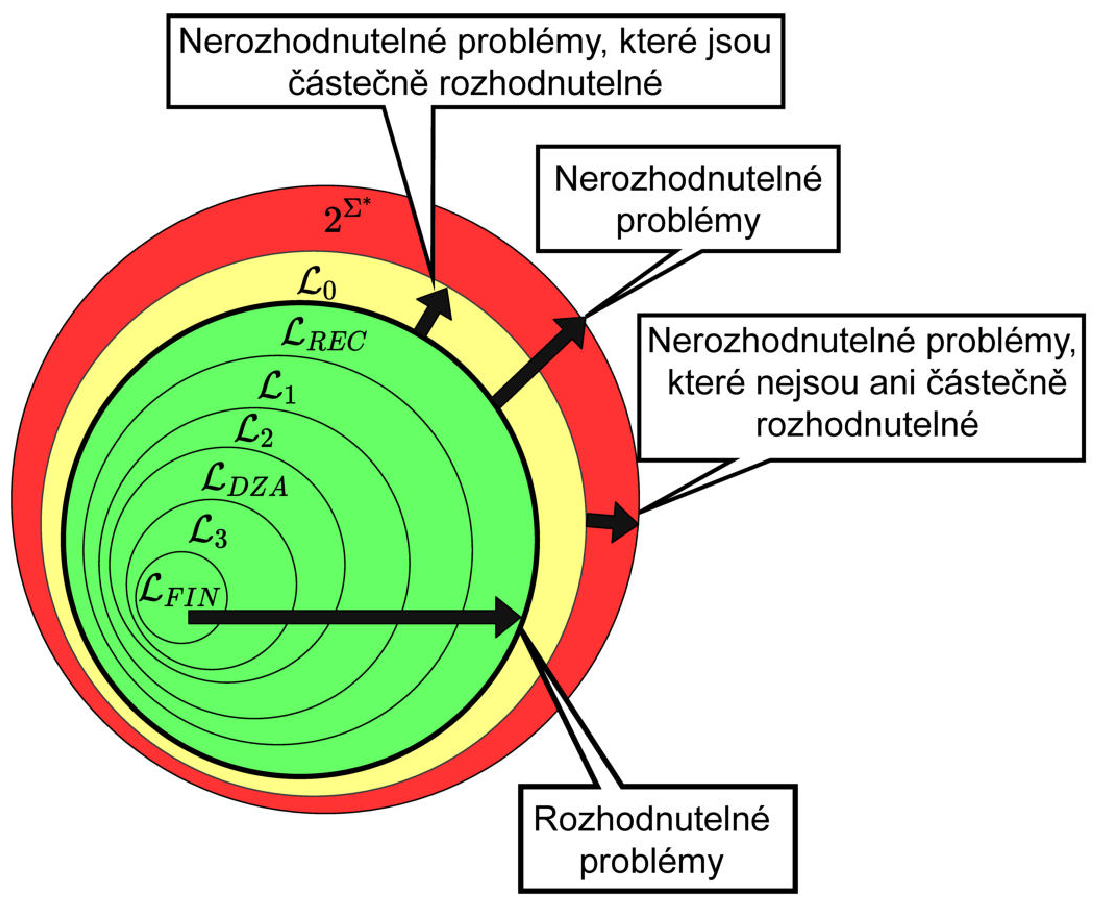
\includegraphics[width=0.9\linewidth]{fj_hierarchy.pdf}
    \caption{Hierarchie jazýků/problémů a jejich (ne)rozhodnutelnost.}
\end{figure}

%%%%%%%%%%%%%%%%%%%%%%%%%%%%%%%%%%%%%%%%%%%%%%%%%%%%%%%%%%%%%%%%%%%%%%%%%%%%%%%%

\section{Známé problémy}

\paragraph*{Problém zastavení TS} \begin{compactitem}
    \item Problém zastavení TS $M$ na daném vstupu $w$ (HP, \textit{Halting Problem}).

    \item Neformálně: Znáte-li zdrojový kód programu (TS) a jeho vstup, rozhodněte, zda program zastaví, nebo zda poběží navždy bez zastavení.

    \item Problém není rozhodnutelný, ale je částečně rozhodnutelný.
\end{compactitem}

$$ HP = \{ \langle M \rangle \# \langle w \rangle ~|~ \text{TS M na vstupu w zastaví} \} $$

\paragraph*{Problém nezastavení TS} \begin{compactitem}
    \item Problém nezastavení TS $M$ na daném vstupu $w$ (co-HP, \textit{co-Halting Problem}).

    \item Neformálně: Znáte-li zdrojový kód programu (TS) a jeho vstup, rozhodněte, zda program nezastaví (poběží navždy bez zastavení), nebo zda zastaví.

    \item Problém není ani částečně rozhodnutelný.
\end{compactitem}

$$ coHP = \{ \langle M \rangle \# \langle w \rangle ~|~ \text{TS M na vstupu w nezastaví} \} $$

\paragraph*{Problém náležitosti} \begin{compactitem}
    \item Problém náležitosti řetězce $w$ do jazyka $L$, $L \in \mathcal{L}_0$ (MP, \textit{Membership Problem}).

    \item Neformálně: Znáte-li TS a jeho vstup, rozhodněte, zda TS daný vstup přijme (zastaví a akceptuje) a nebo nepřijme (zastaví a neakceptuje, zastaví abnormálně, nezastaví).

    \item Problém není rozhodnutelný, ale je částečně rozhodnutelný.
\end{compactitem}

$$ MP = \{ \langle M \rangle \# \langle w \rangle ~|~ \text{M je TS, který akceptuje řetězec w} \} $$

%%%%%%%%%%%%%%%%%%%%%%%%%%%%%%%%%%%%%%%%%%%%%%%%%%%%%%%%%%%%%%%%%%%%%%%%%%%%%%%%

\section{Diagonalizace}

Spočetné -- umím spočítat a uspořádat. Existuje bijekce mezi množinou N a každou spočetnou množinou. Dokážu namapovat.

Jazyků je nespočetně mnoho.

Ale všech možný programů (TS) je spočetně mnoho, proč? Protože kódování TS je možné interpretovat jako přirozené číslo. A těch je spočetně mnoho.

\todo{todo}

todo dukaz Existence jazyků mimo třídu 0

K porovnávání mohutnosti dvou množin

Technika důkazu, že nějaký problém není rozhodnutelný (částečně rozhodnutelný)

%%%%%%%%%%%%%%%%%%%%%%%%%%%%%%%%%%%%%%%%%%%%%%%%%%%%%%%%%%%%%%%%%%%%%%%%%%%%%%%%

\section{Redukce}

\begin{compactitem}

    \item Problém je aspoň tak těžkej jako jinej problém

    \item Vytváří uspořádání na problémech, nějaký problém je aspoň tak těžký jak jiný problém

    \item Redukce jazyka A na jazyk B je totální, rekurzivně vyčíslitelná funkce... (To znamená, že je implementovatelné pomocí úplného TS)

    \item Zachovává členství.

    \item Existuje-li redukce jazyka $A$ na $B$, říkáme, že $A$ je redukovatelný na $B$, což značíme $A \leq B$.

\end{compactitem}

\todo{todo}

Jde o podobný případ jako problém zastavení TS, s tím rozdílem, že po zastavení je ještě třeba zjistit, zda zastavil normálně a přijal a nebo abnormálně.

\paragraph*{Redukce MP na HP}

$$ HP \leq MP $$

$$ \sigma(\langle M \rangle \# \langle w \rangle) = \langle M' \rangle \# \langle w' \rangle$$

%%%%%%%%%%%%%%%%%%%%%%%%%%%%%%%%%%%%%%%%%%%%%%%%%%%%%%%%%%%%%%%%%%%%%%%%%%%%%%%%

\section{Postův korespondenční problém}

\todo{todo}
